% !TEX root = main_org.tex


\chapter{Experimental setup}
\section{Large Hardon Collider}

The Large Hadron Collider is the biggest accelerator in the world which wasbuilt between 2002 and 2009 at CERN. This powerful  particle accelerator was installed in the 27km long circular underground tunnel across the border between France and Swiss. It has 16 RF(radio frequency) accelerating cavities and over 1600 superconducting magnets. With this accelerator, we can collide protons with a centre-of mass energy up to 14 TeV and Pb ions with a centre-of mass energy per nucleon up to 5.5 TeV \cite{lhc}.

The protons are first accelerated in linear accelerator LINAC and injected into the BOOSTER at an energy of 50 MeV. The BOOSTER accelerates them to 1.4 GeV before they are sent to the Proton Synchrotron (PS), which further accelerates the protons to 25 GeV.  From the PS they are sent to the Super Proton Syncrotron (SPS), where they yet again are accelerated, this time to 450 GeV. Finally they are transferred to the LHC ring. At Maximum the 2808 bunches of the protons traevel the ring either clockwise or counter- clockwise.

Procedures for operating the LHC with lead ions are similar, though with some differences. The lead ions are produced by heating a highly purified lead sample up to around 550$^\circ$. This creates a number of charge states, with Pb$^{27+}$ being the dominant one. The ions are accelerated in LINAC 3 to 4.2 MeV per nucleon. Afterwards they are sent through a carbon foil, which strips them to Pb$^{54+}$.  The Pb$^{54+}$ beam is leaded to the Low Energy Ion Ring (LEIR), where it is accelerated to 72 meV per nucleon, before being transferred to the PS. At the PS, the ions are accelerated up to 5.9 GeV per nucleon. The ions once again are sent through the foil, stripping them to Pb$^{82+}$, which is the final ionization used for collisions. After the PS the now fully stripped ions arrive at the SPS, where they are accelerated to 177 GeV per nucleon, before being sent into the LHC ring for acceleration to their collision energy($0.999999991c$ at $\sqrt{s_{NN}}=7$TeV). As in the proton case, the ion bunches are sent either clockwise or counter-clockwise around the ring. The collision of lead ions only occur at 3 of the experiment sites, namely ALICE \cite{alice}, ATLAS \cite{atlas}, and CMS \cite{cms}. The ATLAS and CMS experiments are general purpose detectors used to look for signs of new physics, including the origins of the mass of elementary particles and extra dimensions. The ALICE detector is designed to study the properties of the so called quark gluon plasma (QGP) which is believed to have been created in the first microseconds after the Big Bang. Details will be discussed in the following chapter.


     \begin{figure}[!h]
		\begin{center}
        	\resizebox{0.85\columnwidth}{!}{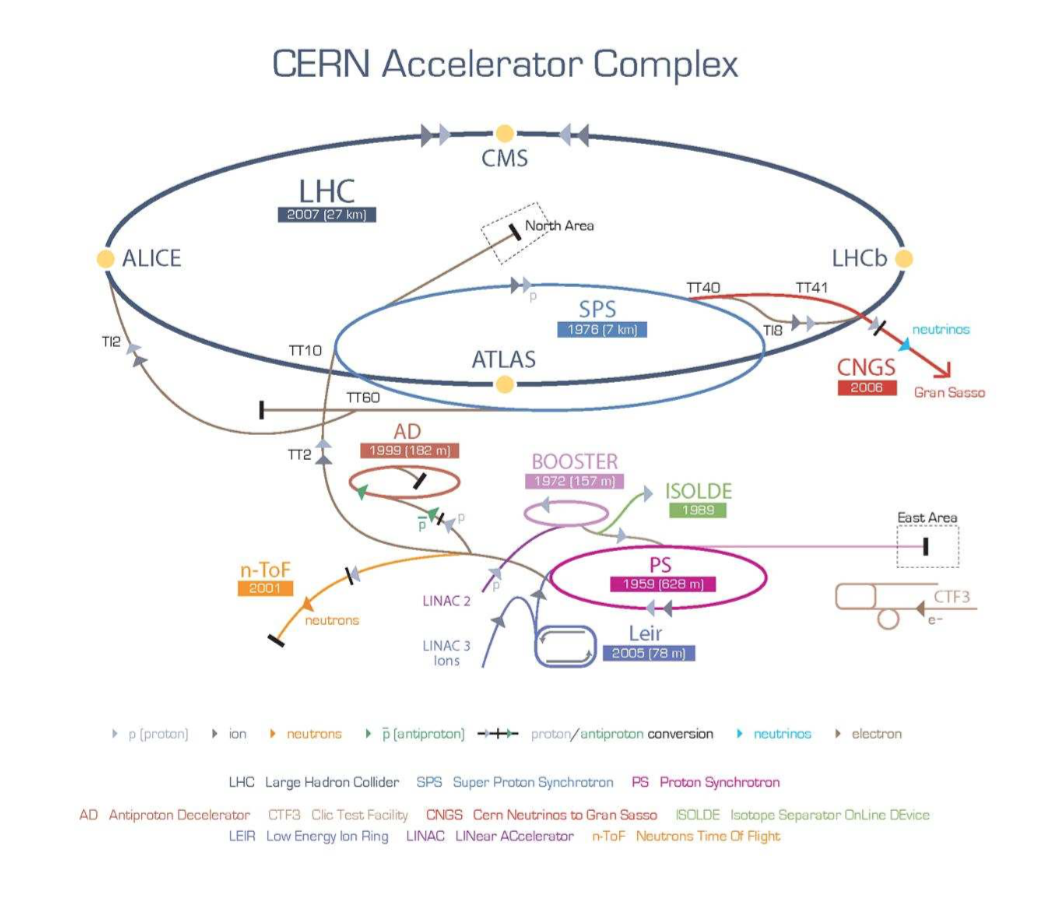
\includegraphics{figures/lhc}}
        	\caption{Schematic view of Large Hadron Collider}
        	\label{lhc}
        \end{center}
    \end{figure}


\section{The ALICE experiment}

ALICE (A Large Ion Collider Experiment) is one of the experiments placed in LHC. The collaboration involves more than a thousand scientists and engineers from 116 institutes and 33 countries. It was designed to study the properties of QCD and to characterize the Quark-Gluon Plasma (QGP). It is the only experiment at LHC which was optimized for the heavy ions collisions.


     \begin{figure}[!h]
		\begin{center}
        	\resizebox{0.85\columnwidth}{!}{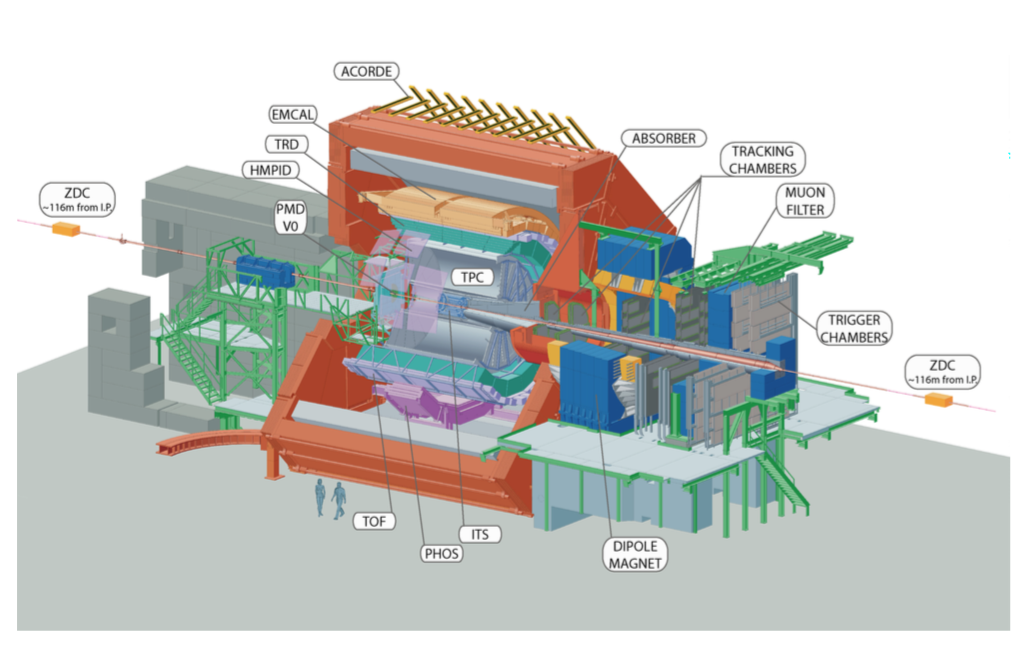
\includegraphics{figures/alice}}
        	\caption{Schematic view of ALICE detector \cite{cds}}
        	\label{alice}
        \end{center}
    \end{figure}

The detector is placed in the solenoid magnet from the L3 experiment. This provides a relatively low magnetic field of 0.5 T, which allows to measure low momentum particles corresponding to the so-called soft QCD, as well a s more energetic particles from hard processes. Because of the extremely high multiplicity expected in nucleus-nucleus collisions at LHC energies, the design of ALICE was optimized for a multiplicity $dN_{ch}/dy = 8000$. ALICE has an efficient and robust tracking system over a large momentum range, from tens of MeV/$c$ (soft physics) to over 100 GeV/$c$ (jet physics). As some of the tracking detectors are based on drift technologies, they are slower then the detectors operated by the other LHC experiments but can work at the nominal LHC ion beam rate of 10 kHz. A specificity of the ALICE detector over the other LHC experiments is its emphasis on hadron and lepton identification (PID). It is achieved over much of the momentum range using most known PID techniques, such as $dE/dx$ energy loss, time-of-flight, transition and Cherenkov radiation, electromagnetic calorimetry, muon filters, and topological decay reconstruction.

The detectors in the ALICE experiment are arranged in a classical layered structure around the interaction point as Shown in Figure.\ref{alice}. Here is a short description of the main detectors which used in this analysis. Most of description here are taken from the ALICE Technical Design Report (ALICE TDR) \cite{Cortese:879894}, and more detail information can be found in CERN document system (CDS) \cite{cds}.



\subsection{ITS}

The Inner Tracking System (ITS) consists of six layers of silicon detectors with radii few cm as shown Figure.\ref{its}

     \begin{figure}[!h]
		\begin{center}
        	\resizebox{0.85\columnwidth}{!}{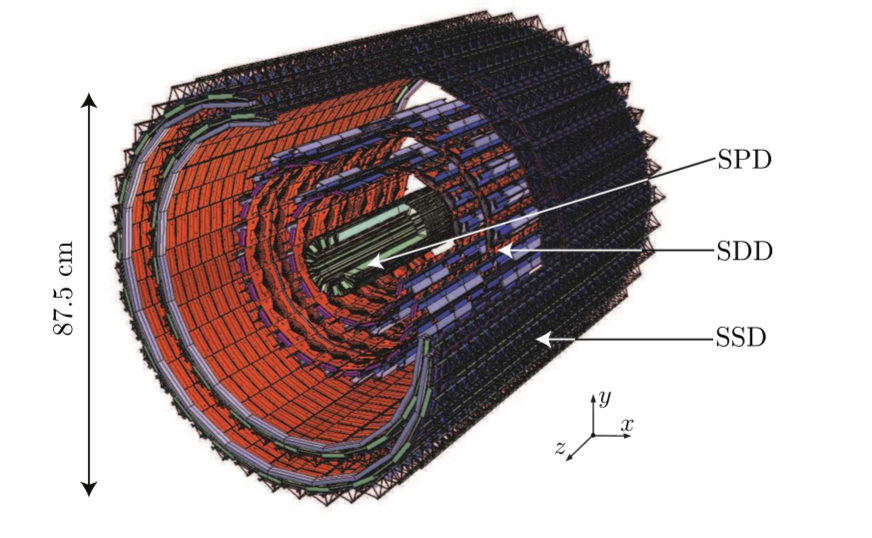
\includegraphics{figures/its}}
        	\caption{ALICE Inner Tracking System(ITS), includes Silicon Pixel Detector(SPD) and Silicon Drift Detector(SDD) and Silicon Strip Detector(SSD)}
        	\label{fig:its}
        \end{center}
    \end{figure}


The main purpose of the ITS is the reconstruction of the primary vertex of the collision as well as the reconstruction of secondary vertexes with a resolution better than 100 $\mu$m in transverse direction. The ITS stand-alone tracking can provide the tracking information for low-momentum particles that do not reach the TPC. The $p_T$ cut-off at nominal field for the two innermost layers is about 35 MeV/c.

The two innermost layers, Silicon Pixel Detector (SPD) \cite{Meddi200140}, are based on hybrid silicon pixels which consist of silicon detector diodes with a thickness of 200 $\mu$m. The first layer and the second layer are placed at 3.9 cm and 7.6 cm with an acceptance of $|\eta| < 2.0$ and $|\eta| < 1.4$, respectively. The SPD has approximately 10 million channels. The pixel readout chip (ALICE1LHCb) is a mixed- signal ASIC for the readout of 8192 pixels. Each pixel cell contains a preamplifier-shaper with leakage current compensation, followed by a discriminator. A signal above threshold results in a logical 1 which is propagated through a delay line during the 6 $\mu$s latency time until the arrival of the L1 trigger signal. Upon arrival of the L1 trigger, the logical level present at the end of the delay line is stored in the first available buffer location. The outputs of the discriminators in the pixel cells of the ALICE1LHCb chip provide a fast-OR digital pulse when one or more pixels are hit on the chip. 

The third and forth layer, Silicon Drift Detector (SDD) \cite{Alessandro:2010rq}, consist of a 300 $\mu$m thick layer of homogeneous high-resistivity silicon. The readout of the SDD is analog, therefore particle identification can be conducted using the information of energy-loss. The SDD has 133,000 channels.

The two outermost layers, Silicon Strip Detector (SSD) \cite{Contin:2011rs}, consist of sensors equipped on both sides with silicon micro-strips. These are arranged under a stereo angle of 35 mrad allowing for a two-dimensional measurement of the track position together with an energy-loss measurement for particle identification. The SSD has approximately 2.6 million channels \cite{Contin:2009lza}.



\subsection{TPC}

The Time Projection Chamber (TPC) \cite{CERN-LHCC-2013-020} is the main tracking device of the ALICE experiment. It is a large cylinderical gas chamber detector with $\sim 88$m$^3$ volume in 0.5 T solenoidal magnetic filed parallel to the E field. 

This detector is designed to have $dE/dx$ resolution better than 5\% and a relative $p_T$ resolution better than 1\% for momenta of $\sim 1$GeV/$c$ and better than 2.5\% for momenta of 4GeV/$c$, and two track resolution capable of separating tracks with a relative momentum difference of $< 5$MeV.

The TPC is separated by two volumes with the Central Electrode (CE) made of single stretched Mylar foil, and secondary electrons drift toward the end-caps. 

\begin{figure}[!p]
\centerline{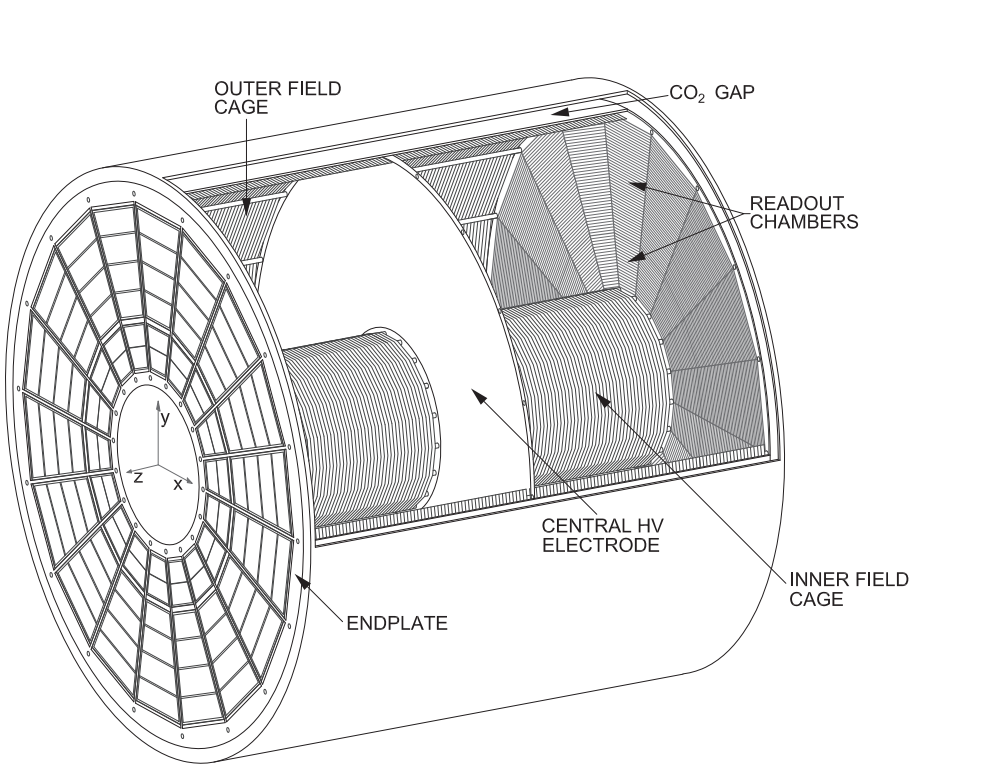
\includegraphics[width=10.0cm]{figures/tpc1}}
\centerline{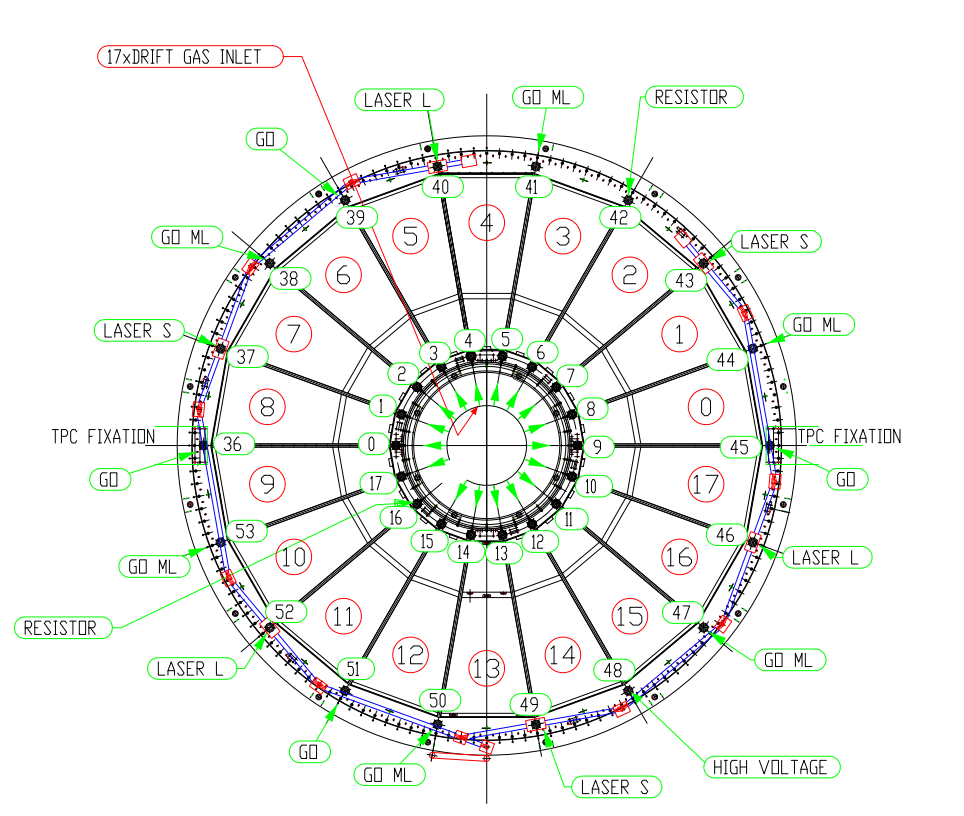
\includegraphics[width=10.0cm]{figures/tpc2}}
\caption{ ALICE Time Projection Chamber } 
\label{fig:cmsevt}
\end{figure}


Volumes are filed with Ne-CO$_2$-N$_2$ (90\%-10\%-5\%) gas which is optimized for drift speed, ion mobility, and low diffusion of electrons. Since, Ne-CO$_2$-N$_2$ gas have dependence of drift velocity on temperature, TPC is aiming for a thermal stability with $\Delta T < 0.1$K in the drift volume over the running period. 

As the gas detector, the TPC field cage has to be operated at very high voltage gradients, of about 400V/cm, with a high voltage of 100kV at the central electrode which results in a maximum drift time of about 90$\mu$s.

The TPC covers a pseudo-rapidity range of $|\eta| < 0.9$ for full track length within the TPC volume. Also it provides 0 to $2\pi$ azimuthal coverage except for the dead zones in the TPC, and it makes the TPC an ideal detector for anisotropic flow analysis, since these inefficiencies in the  azimuthal acceptance would result in non-negligible systematic biases for the azimuthal angle correlations analysis.



\subsection{VZERO}

The VZERO detectors(also often called V0) \cite{collaboration2013performance} are designed with a much larger acceptance, in order to perform as a minimum bias trigger in both proton-proton and Pb–Pb collisions. Furthermore, it is also used, together with the timing information of the collision, for the rejection of beam-gas interactions. The VZERO is also used to determine the event centrality and many of ALICE analyses use centrality determination from VZERO.

\begin{figure}[!h]
		\begin{center}
        	\resizebox{0.85\columnwidth}{!}{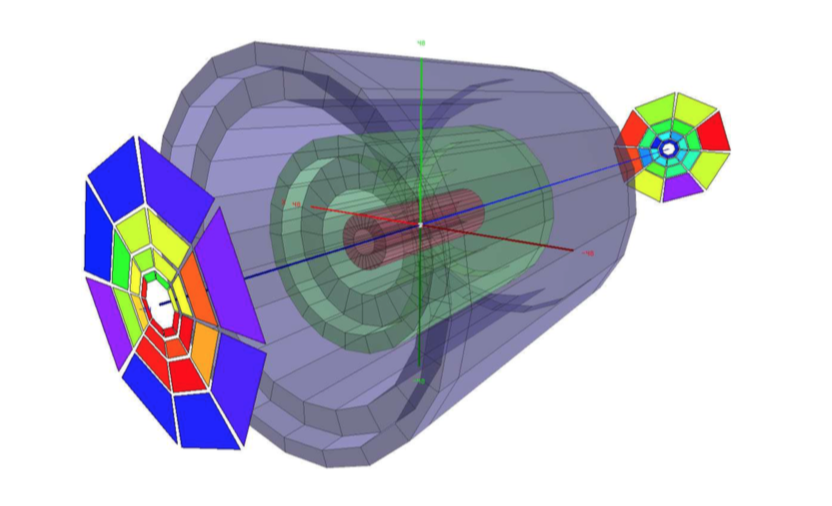
\includegraphics{figures/v0}}
        	\caption{ALICE VZERO detectors on both side of TPC}
        	\label{its}
        \end{center}
    \end{figure}


This consists of two separate arrays of scintillator counters and V0A and V0C, placed on different sides of the central barrel detectors along the beam line. V0A/C are placed asymmetrically with respect to the interaction point. V0A is located 340 cm from the interaction point on the side opposite to the muon arm, while V0C is placed 90 cm from the interaction point on the opposite side from V0A. Because of this asymmetry, V0A and V0C have different pseudo-rapidity coverage. The V0A covers pseudo-rapidity range $2.8 < \eta < 5.1$, while V0C covers $-3.7 < \eta < -1.7$.

The V0A/V0C are segmented into 32 elementary counters distributed in four rings. Each ring covers 0.4-0.6 unit of pseudo-rapidity. The rings are divided into eight sectors of 45$^{\circ}$. The elementary counter consists of scintillator material with embedded WaveLength Shifting (WLS) fibers. The light from the WLS is collected by clear fibers and transported to PhotoMultiplier (PM) installed at 3-5 m from the detectors, inside the L3 magnet. The time resolution of each individual counter will be better than 1 ns.

Signals from each PMT are sent to an electronics circuit, which delivers two signals. The first one is sent to a threshold discriminator for the generation of the V0 event triggers. It is amplified by a factor of about 10. If at least one discriminator is fired during the time window around the timing of the beam crossing (after 3 ns for V0A, 11 ns for V0C), the V0 event trigger is issued.

\subsection{Other detectors}

\subsubsection{TRD}
Transition Radiation Detector (TRD) \cite{Cortese:519145} is placed from 2.9 to 3.8 m from the interaction point. It discriminates electrons from pions with high efficiency for momenta about 1 GeV/$c$ by the identification of the transition radiation photons from electrons. Also this detector can provide the trigger signals for electron 

\subsubsection{TOF}
Time Of Flight (TOF) \cite{alici2013mrpc} is made of Multigap Resistive Plate Chamber strips (MRPC), which are made by a ten layer double-stack detector with a time resolution of about 40 ps. By measuring the time particles take to reach it, and combined with the tracking information of the TPC, it allows for the identification of pions, kaons and protons

\subsubsection{HMPID}
High Momentum Particle Identification Detector (HMPID) \cite{Molnar:2008pr} consists of an array of proximity-focusing Ring Imaging CHerenkov counters (RICH) and covers a pseudo-rapidity range of $|\eta| < 0.6$ and 58$^{\circ}$ of azimuthal angle. The HMPID discriminates pions and kaons in the range $1<p_T<3$GeV/$c$ and protons and kaons in the range $2<p_T<5$GeV/$c$ by means of their Cherenkov rings.

\subsubsection{PHOS}
PHOton Spectrometer (PHOS) \cite{1742-6596-160-1-012045}  is placed partially opposite to the EMCAL and made of highly segmented electromagnetic calorimeter of lead-tungstenate (PbWO4 , PbWO) crystals with a radiation length of 20X$_0$. It is used for neutral mesons and direct photon measurements.

\subsubsection{EMCAL}
ElectroMagnetic Calorimeter (EMCAL) \cite{rene2010alice} is a lead scintillator sampling calorimeter that covers an azimuthal angle range of 107$^{\circ}$ in the rapidity interval $|\eta|<0.7$ at a radial distance of about 4.5 m from the vacuum tube. The EMCAL is designed for the study of jet-physics and can provide trigger signals for hard jets, photons and electrons.

\subsubsection{Muon Spectrometer}

Muon Sepctrometer is situated in the forward($-4 < \eta < -2.5)$) region on one side of the experiment. It track muons with momentum $p > 4$GeV/$c$. And used for the analaysis of quarkonia decaying to the $\mu\mu$.

\subsubsection{TZERO}

TZERO (T0) \cite{cortese2004alice} detector is designed to determine the collision time. T0 consists of two units, one on each side of the interaction point. Each T0 unit is comprised of quartz Cherenkov radiators glued to photo multiplier tubes. A coincidence between signals in both sides is used for both vertex and time determination


\subsubsection{Zero Degree Calorimeter}

The Zero Degree Calorimeters (ZDC) \cite{oppedisano2009physics} are positioned at extremely forward angles. Their role is to measure the spectator nucleons from heavy ion collisions, in order to estimate the number of participants, and hence the centrality. Furthermore they are also used to determine the event plane. 

\subsection{Analysis Framework}

 The ROOT system is an object-oriented framework (written in C++) developed at CERN in the 90’s and used by various collaborations worldwide as a starting framework on top of which the specific framework needed for particular collaboration is being built. It provides a full set of features needed for event generation, detector simulation, event reconstruction, data acquisition and data analysis. All features are encoded in a set of about 650 classes grouped in about 40 libraries. A vast majority of ROOT classes inherit from the common base class called TObject, which provides default behavior and protocol (e.g. protocol for the object I/O, error handling, sorting, inspection, printing, drawing, etc.) for all objects in the ROOT system, but the standalone classes which can be used as built-in types are also implemented. 

The AliRoot is the specific version of framework which built on the ROOT system. It's optimized for ALICE simulation, alignment, calibration, reconstruction, visualization, quality assurance, and analysis. Most of codes are written in C++ and some parts are written in Fortran.


\begin{figure}[t]
\centerline{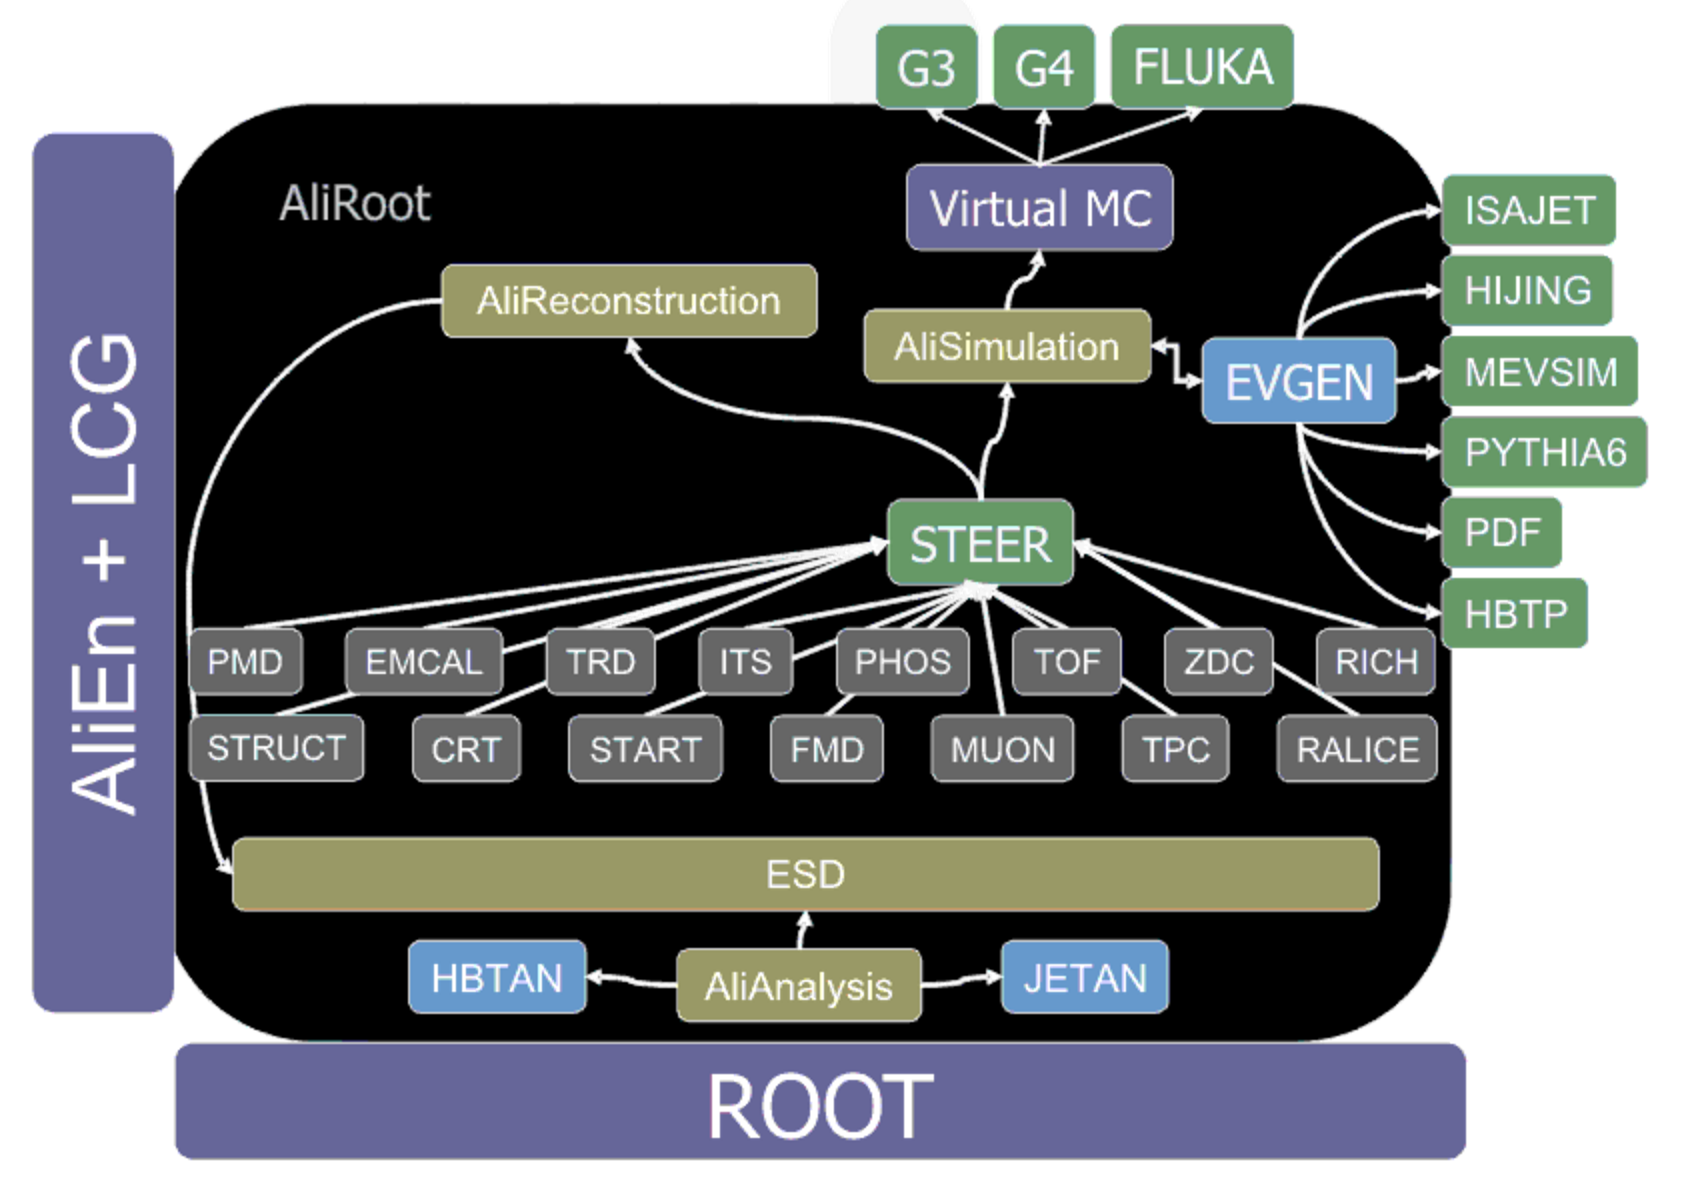
\includegraphics[width=12.0cm]{figures/aliroot}}
\caption{Picture of general schema of the AliRoot architecture \cite{aliroot}} 
\label{fig:cmsevt}
\end{figure}



Also for the large consumption of CPU power, the ALICE analysis framework provides several distributed computing systems, including the parallel computing (PROOF) or, Grid.  Because of the huge amount of data produced by the ALICE detector ($\sim$ 2PB per year) \cite{1742-6596-219-7-072023}, the reconstructed events are saved into a worldwide computing center. The computing center has a distributed hierarchy with Tier 0 to Tier 3, and the ALICE Virtual Organization (ALICE VO) is made of more than 80 sites. Each site provides large computing power with physical machines where the software programs can be run. By using JDL(Job Description Language) and XML(eXecutable Machine Language), users can use codes with AliRoot over 1500 CPUs at the same time.